\documentclass[11pt]{article}

\usepackage{times}
\usepackage{epsf}
\usepackage{epsfig}
\usepackage{amsmath, alltt, amssymb, xspace}
\usepackage{wrapfig}
\usepackage{fancyhdr}
\usepackage{url}
\usepackage{verbatim}
\usepackage{fancyvrb}
\usepackage{float}

\usepackage{subfigure}
\usepackage{cite}
\usepackage{hyperref}
\hypersetup{%
    pdfborder = {0 0 0}
}
\topmargin      -0.50in  % distance to headers
\oddsidemargin  0.0in
\evensidemargin 0.0in
\textwidth      6.5in
\textheight     8.9in 


%\centerfigcaptionstrue

%\def\baselinestretch{0.95}


\newcommand\discuss[1]{\{\textbf{Discuss:} \textit{#1}\}}
%\newcommand\todo[1]{\vspace{0.1in}\{\textbf{Todo:} \textit{#1}\}\vspace{0.1in}}
\newtheorem{problem}{Problem}[section]
%\newtheorem{theorem}{Theorem}
%\newtheorem{fact}{Fact}
\newtheorem{define}{Definition}[section]
%\newtheorem{analysis}{Analysis}
\newcommand\vspacenoindent{\vspace{0.1in} \noindent}

%\newenvironment{proof}{\noindent {\bf Proof}.}{\hspace*{\fill}~\mbox{\rule[0pt]{1.3ex}{1.3ex}}}
%\newcommand\todo[1]{\vspace{0.1in}\{\textbf{Todo:} \textit{#1}\}\vspace{0.1in}}

%\newcommand\reducespace{\vspace{-0.1in}}
% reduce the space between lines
%\def\baselinestretch{0.95}

\newcommand{\fixmefn}[1]{ \footnote{\sf\ \ \fbox{FIXME} #1} }
\newcommand{\todo}[1]{
\vspace{0.1in}
\fbox{\parbox{6in}{TODO: #1}}
\vspace{0.1in}
}

\newcommand{\mybox}[1]{
\vspace{0.2in}
\noindent
\fbox{\parbox{6.5in}{#1}}
\vspace{0.1in}
}


\newcounter{question}
\setcounter{question}{1}

\newcommand{\myquestion} {{\vspace{0.1in} \noindent \bf Question \arabic{question}:} \addtocounter{question}{1} \,}

\newcommand{\myproblem} {{\noindent \bf Problem \arabic{question}:} \addtocounter{question}{1} \,}


\newcommand{\copyrightnotice}[1]{
\vspace{0.1in}
\fbox{\parbox{6in}{
      This lab was developed for the Labtainer framework by the Naval Postgraduate
      School, Center for Cybersecurity and Cyber Operations under sponsorship from
      the DoD CySP program.  This work is in the public domain, and cannot be copyrighted.}}
\vspace{0.1in}
}


\newcommand{\idea}[1]{
\vspace{0.1in}
{\sf IDEA:\ \ \fbox{\parbox{5in}{#1}}}
\vspace{0.1in}
}

\newcommand{\questionblock}[1]{
\vspace{0.1in}
\fbox{\parbox{6in}{#1}}
\vspace{0.1in}
}


\newcommand{\argmax}[1]{
\begin{minipage}[t]{1.25cm}\parskip-1ex\begin{center}
argmax
#1
\end{center}\end{minipage}
\;
}

\newcommand{\bm}{\boldmath}
\newcommand  {\bx}    {\mbox{\boldmath $x$}}
\newcommand  {\by}    {\mbox{\boldmath $y$}}
\newcommand  {\br}    {\mbox{\boldmath $r$}}


\newcommand{\tstamp}{\today}   
%\rfoot[\fancyplain{\tstamp} {\tstamp}]  {\fancyplain{}{}}

\pagestyle{fancy}
\lhead{\bfseries Labtainers}
\chead{}
\rhead{\small \thepage}
\lfoot{}
\cfoot{}
\rfoot{}




\begin{document}

\begin{center}
{\LARGE NetFlow Record Analysis}
\vspace{0.1in}\\
\end{center}

\section{Overview}
As you learned in the \textit{pcap-lib} lab, packet traces can be large. The ≈ 2 GB trace file from that lab was actually quite small. Consider capturing all of the packets on a high-speed Internet backbone link, or at an enterprise border router (the ingress/egress point for campus traffic) for any extended period of time!
However, some traffic analysis tasks do not require the fine granularity of pcap, i.e. do not need details such as individual packet timing, payload contents, etc. Instead, flow records capture many relevant properties of traffic while using less storage capacity, impose different capture processing requirements, etc.
By “flow” we are referring to the aggregate of all packets belonging to a connection. A flow is defined as all packets with a common 5-tuple:
<IP Src, IP Dst, Protocol, Src Port, Dst Port>
This lab explores “NetFlow.” NetFlow is a protocol and data record type\footnote{See RFC3954: http://tools.ietf.org/html/rfc3954}
, first developed by Cisco. NetFlow has matured and evolved into the IP Flow Information Export (IPFIX) standard as specified in http://tools.ietf.org/html/rfc7011. All commercial routers (and even dd-wrt, openwrt, etc.) support some version of IPFIX collection and export \footnote{See, for instance: http://www.cisco.com/c/en/us/td/docs/ios-xml/ios/fnetflow/configuration/xe-3s/ fnf-xe-3s-book/fnf-ipfix-export.html}.
Future labs build on the concepts here – it is imperative that you understand these basics in order to be successful with subsequent lab work.
There are 23 questions in the lab. 

\subsection {Background}
The student is expected to have completed the {\tt pcap-lib} lab.

\section{Lab Environment}
\label{environment}
This lab runs in the Labtainer framework,
available at http://nps.edu/web/c3o/labtainers.
That site includes links to a pre-built virtual machine
that has Labtainers installed, however Labtainers can
be run on any Linux host that supports Docker containers.

From your labtainer-student directory start the lab using:
\begin{verbatim}
    labtainer netflow
\end{verbatim}
\noindent A link to this lab manual will be displayed.  

The home directory of the resulting computer contains a directory named {\tt mystuff}.  That directory is shared with your Labtainers host,
at:
\begin{verbatim}
   labtainer-student/mystuff
\end{verbatim}
\noindent Files and directories that you create in {\tt mystuff} will persist independent of this lab (and other labs that make the mystuff
directory available).  Consider placing your code and scripts there.
\section{Tasks}  
\subsection{Understanding IPFIX (25 pts)}
We'll start by more carefully understanding IPFIX and flow records.
\begin{enumerate}
\item {[2 pts]} Under what conditions is a flow “expired,” i.e. when are the statistics for a particular flow exported as an IPFIX record?
\item {[2 pts]} What transport protocol does IPFIX use to export records to remote IPFIX collection servers?
\item {[2 pts]} Do IPFIX records represent bidirectional or unidirectional captured traffic? Explain your answer.
\item {[2 pts]} Visit a popular web site, e.g. http://www.cnn.com/ and capture the packets as a pcap file (using Wireshark or tcpdump). How many flows are generated as part of your session with the web site?
\item {[2 pts]} Provide an example of an attack that cannot be detected with IPFIX records, but can be detected by capturing packets (pcap).
\end{enumerate}
Consider a hypothetical 1Gbps Ethernet link on which you would like to monitor traffic. Assume that the link is 75% utilized and that the only traffic on the link is IP. Assume that the average packet size is 800 bytes.
\begin{enumerate}[resume]
\item {[6 pts]} What is the minimum size of a one-hour pcap capture on the link? State any assumptions necessary.
\item {[5 pts]} Assume that there are an average of 50 packets per flow. Assume that each IPFIX flow record is a fixed 64 bytes. What is the minimum size of a one-hour IPFIX capture on the same link? State any assumptions necessary.
\end{enumerate}
Even with flow aggregation, the number of records may be very large. In addition, the router hardware may not be able to maintain state over all flows or packets transiting the device. As a result, many routers implement flow sampling. If a router is running 1:1000 sampling, then only every 1000th packet is considered for IPFIX processing3.\footnote{This is a very basic form of sampling – we consider other strategies in this lab.}
\begin{enumerate}[resume]
\item {[2 pts]} Provide an example of a traffic monitoring task that cannot be successfully completed with sampled IPFIX. Explain your answer.
\item {[2 pts]} Provide an example of a traffic monitoring task that can be successfully completed with sampled IPFIX. Explain your answer.
\item a very basic form of sampling – we consider other strategies in this lab and future lectures.
\end{enumerate}
 
To better understand IPFIX, we have created an IPFIX capture of the traffic from the {\tt pcap-lib} lab (i.e. it is the same traffic, but stored as IPFIX records).
In order to process the flow records, we will use the CMU SiLK software suite:
   https://tools.netsa.cert.org/silk/
This consists of a number of command-line tools that can be used to answer the questions below. To get started you will want to investigate the useage of \textit{rwaddrcount, rwstats}, and \textit{rwfilter}. You are not required to write any code for this lab, but may choose to do so at your discretion.
Refer to the IPFIX file in {\tt trace2.silk} in your home directory.
Using the available SiLK tools on your system\footnote{See https://tools.netsa.cert.org/silk/docs.html for help}
, answer the following questions:
\begin{enumerate}[resume]
\item {[5 pts]} How many unique IP source addresses are present in the trace?
\item {[5 pts]} How many unique IP destination addresses are present in the trace?
\item {[5 pts]} Do your answers for the number of source and destination addresses agree with those you found in the previous lab? Explain why or why not.
\end{enumerate}
The SiLK tools enable easy and fast analysis of common tasks, without writing specialized programs. Answer the following:
\begin{enumerate}[resume]
\item {[5 pts]} What fraction of the total packet count do the top 10 IP sources represent? 
\item {[5 pts]} What are the top 5 most common destination ports?
\item {[5 pts]} What are the top 5 most common source ports?
\end{enumerate}
Recall that the IPFIX capture represents the same traffic as the pcap capture from the {\tt pcap-lib} lab.
\begin{enumerate}[resume]
\item {[5 pts]} Is the IPFIX file smaller or larger than the pcap capture? Is this what you expect? Explain your answer.
\end{enumerate}
  
George P. Burdell is a network engineer at Haywood Jabuzoff Networks (HJN). George receives a peering request from Alice at Royal Payne Networks (RPN). Recall that two networks will connect to each other and engage in settlement-free peering, where no money is exchanged, when it is mutually beneficial\footnote{For a detailed exposition of Internet peering, see: \url{http://www.akamai.com/dl/technical\_publications/growing\_complexity\_of\_internet.pdf}}.
The topology under consideration is shown in figure \ref{fig:topology}


George’s task is to determine the potential benefit of peering with RPN. To make a quantitative assessment, he collects IPFIX flow records at his border router connecting to his provider (AT\&T), i.e. he monitors traffic between HJN and AT\&T. After one hour, he obtains the following IPFIX found at peering2.silk in your home directory.
To begin, George looks at the following questions:
\begin{enumerate}[resume]
\item {[5 pts]} How many unique IP source addresses are present?
\item {[5 pts]} How many unique IP destination addresses are present?
\item {[5 pts]} What is the minimum, median, and maximum number of bytes per flow? 
\item {[5 pts]} What is the minimum, median, and maximum number of packets per flow? 
\item {[8 pts]} What fraction is TCP traffic of the total byte count?
\end{enumerate}
                 
Many factors are considered in making peering decisions, including the topological footprint of the ISP, traffic symmetry, traffic volume, etc. Help George determine whether to peer with RPN:
\begin{enumerate}[resume]
\item {[7 pts]} RPN owns and advertises the IPv4 prefix: 18.128.0.0/9. What fraction of HJN’s current traffic to AT\&T would instead transit the peering link to RPN if they were to peer?
\item {[5 pts]} Should HJN peer with RPN? Explain your answer in sufficient detail such that your boss understands.
\end{enumerate}

\begin{figure}[H]
\begin{center}
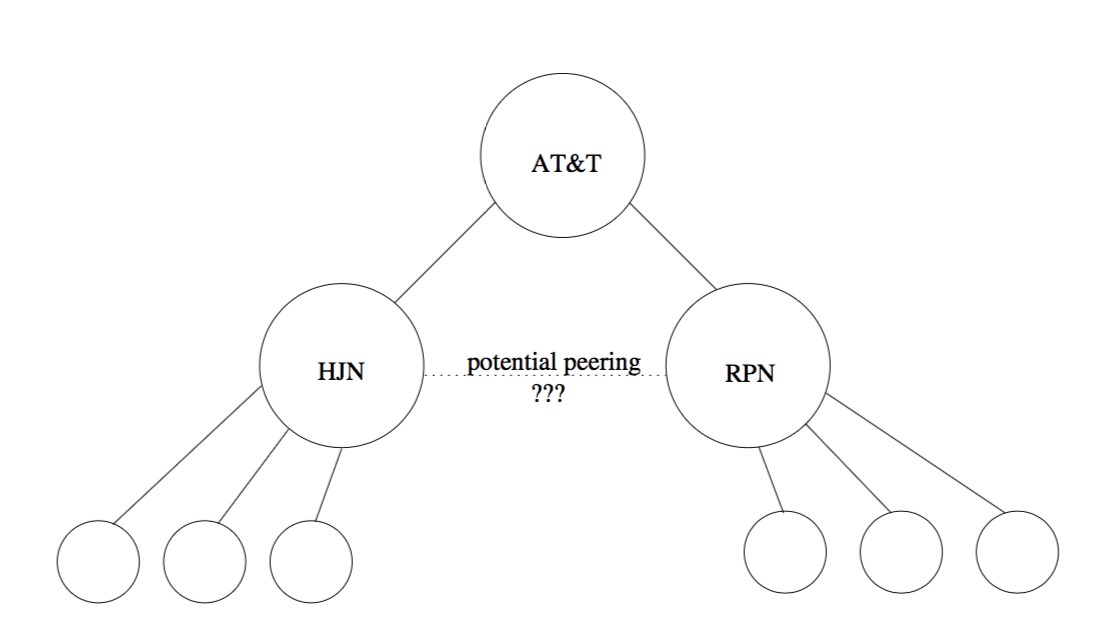
\includegraphics [width=0.8\textwidth]{pic.png}
\end{center}
\caption{Peering topology}
\label{fig:topology}
\end{figure}
\section{Submission}
After finishing the lab, go to the terminal on your Linux system that was used to start the lab and type:
\begin{verbatim}
    stoplab 
\end{verbatim}
When you stop the lab, the system will display a path to the zipped lab results on your Linux system.  Provide that file to 
your instructor, e.g., via the Sakai site.
\end{document}
